\documentclass{standalone}
\usepackage{tikz}
\usetikzlibrary{patterns, positioning}
\usepackage[sfdefault]{ClearSans} %% option 'sfdefault' activates Clear Sans as the default text font
\usepackage[T1]{fontenc}

\begin{document}
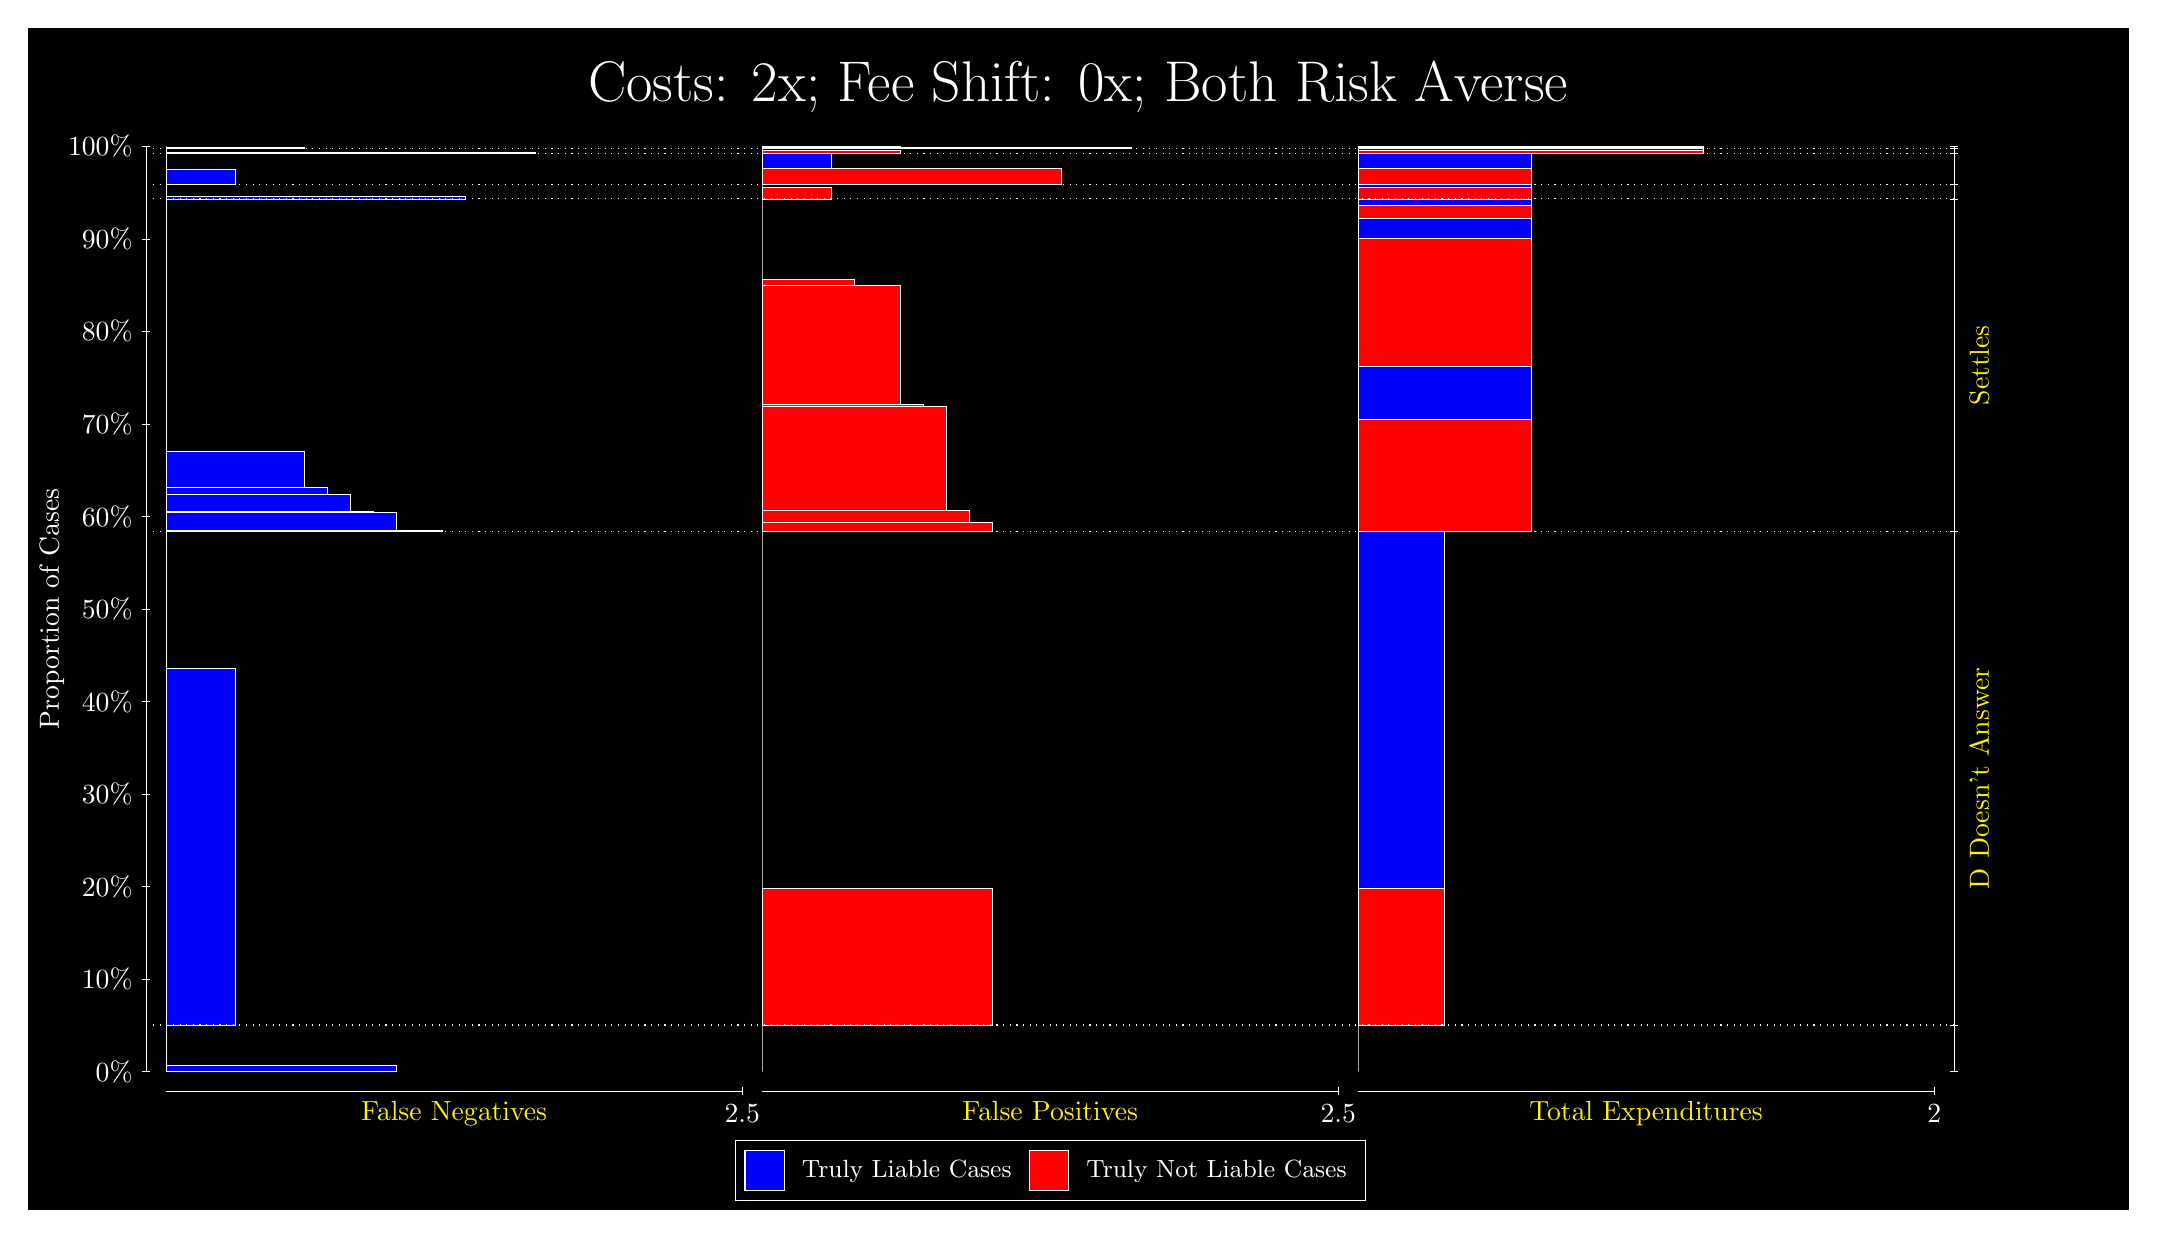
\begin{tikzpicture}
\draw[fill=black] (0,0) rectangle (26.667,15);
\draw[text=white] (0,13.5) rectangle (26.667,15) node[midway] {\huge Costs: 2x; Fee Shift: 0x; Both Risk Averse};
\draw[white, very thin] (1.5,1.75) -- (1.5,13.5);
\node[rotate=90, text=white, anchor=center] at (0.3, 7.625) {Proportion of Cases};
\draw[white, very thin] (1.45,1.75) -- (1.55,1.75);
\node[text=white, anchor=east] at (1.45, 1.75) {0\%};
\draw[white, very thin] (1.45,2.925) -- (1.55,2.925);
\node[text=white, anchor=east] at (1.45, 2.925) {10\%};
\draw[white, very thin] (1.45,4.1) -- (1.55,4.1);
\node[text=white, anchor=east] at (1.45, 4.1) {20\%};
\draw[white, very thin] (1.45,5.275) -- (1.55,5.275);
\node[text=white, anchor=east] at (1.45, 5.275) {30\%};
\draw[white, very thin] (1.45,6.45) -- (1.55,6.45);
\node[text=white, anchor=east] at (1.45, 6.45) {40\%};
\draw[white, very thin] (1.45,7.625) -- (1.55,7.625);
\node[text=white, anchor=east] at (1.45, 7.625) {50\%};
\draw[white, very thin] (1.45,8.8) -- (1.55,8.8);
\node[text=white, anchor=east] at (1.45, 8.8) {60\%};
\draw[white, very thin] (1.45,9.975) -- (1.55,9.975);
\node[text=white, anchor=east] at (1.45, 9.975) {70\%};
\draw[white, very thin] (1.45,11.15) -- (1.55,11.15);
\node[text=white, anchor=east] at (1.45, 11.15) {80\%};
\draw[white, very thin] (1.45,12.325) -- (1.55,12.325);
\node[text=white, anchor=east] at (1.45, 12.325) {90\%};
\draw[white, very thin] (1.45,13.5) -- (1.55,13.5);
\node[text=white, anchor=east] at (1.45, 13.5) {100\%};

\draw[white, very thin] (24.457,1.75) -- (24.457,13.5);
\draw[white, very thin] (24.407,1.75) -- (24.507,1.75);
\node[anchor=west] at (24.407, 1.75) {};
\draw[white, very thin] (24.407,2.3416) -- (24.507,2.3416);
\node[anchor=west] at (24.407, 2.3416) {};
\draw[white, very thin] (24.407,8.6073) -- (24.507,8.6073);
\node[anchor=west] at (24.407, 8.6073) {};
\draw[white, very thin] (24.407,12.832) -- (24.507,12.832);
\node[anchor=west] at (24.407, 12.832) {};
\draw[white, very thin] (24.407,13.016) -- (24.507,13.016);
\node[anchor=west] at (24.407, 13.016) {};
\draw[white, very thin] (24.407,13.408) -- (24.507,13.408);
\node[anchor=west] at (24.407, 13.408) {};
\draw[white, very thin] (24.407,13.47) -- (24.507,13.47);
\node[anchor=west] at (24.407, 13.47) {};
\draw[white, very thin] (24.407,13.5) -- (24.507,13.5);
\node[anchor=west] at (24.407, 13.5) {};

\draw[white, very thin, fill=blue] (1.75,1.75) rectangle (4.6775,1.8287);
\draw[white, very thin, fill=red] (1.75,1.8287) rectangle (1.75,2.3416);
\draw[white, very thin, fill=blue] (1.75,2.3416) rectangle (2.6283,6.8654);
\draw[white, very thin, fill=red] (1.75,6.8654) rectangle (1.75,8.6073);
\draw[white, very thin, fill=blue] (1.75,8.6073) rectangle (5.2631,8.6195);
\draw[white, very thin, fill=blue] (1.75,8.6195) rectangle (4.6775,8.8549);
\draw[white, very thin, fill=blue] (1.75,8.8549) rectangle (4.3848,8.8632);
\draw[white, very thin, fill=blue] (1.75,8.8632) rectangle (4.092,9.0772);
\draw[white, very thin, fill=blue] (1.75,9.0772) rectangle (3.7993,9.164);
\draw[white, very thin, fill=blue] (1.75,9.164) rectangle (3.5065,9.6222);
\draw[white, very thin, fill=red] (1.75,9.6222) rectangle (1.75,12.832);
\draw[white, very thin, fill=blue] (1.75,12.832) rectangle (5.5558,12.869);
\draw[white, very thin, fill=red] (1.75,12.869) rectangle (1.75,13.016);
\draw[white, very thin, fill=blue] (1.75,13.016) rectangle (2.6283,13.206);
\draw[white, very thin, fill=red] (1.75,13.206) rectangle (1.75,13.408);
\draw[white, very thin, fill=blue] (1.75,13.408) rectangle (6.4341,13.422);
\draw[white, very thin, fill=red] (1.75,13.422) rectangle (1.75,13.47);
\draw[white, very thin, fill=blue] (1.75,13.47) rectangle (3.5065,13.486);
\draw[white, very thin, fill=red] (1.75,13.486) rectangle (1.75,13.5);
\draw[white, very thin, fill=red] (9.3189,1.75) rectangle (9.3189,2.2629);
\draw[white, very thin, fill=blue] (9.3189,2.2629) rectangle (9.3189,2.3416);
\draw[white, very thin, fill=red] (9.3189,2.3416) rectangle (12.246,4.0835);
\draw[white, very thin, fill=blue] (9.3189,4.0835) rectangle (9.3189,8.6073);
\draw[white, very thin, fill=red] (9.3189,8.6073) rectangle (12.246,8.7194);
\draw[white, very thin, fill=red] (9.3189,8.7194) rectangle (11.954,8.8801);
\draw[white, very thin, fill=red] (9.3189,8.8801) rectangle (11.661,10.2);
\draw[white, very thin, fill=red] (9.3189,10.2) rectangle (11.368,10.23);
\draw[white, very thin, fill=red] (9.3189,10.23) rectangle (11.075,11.741);
\draw[white, very thin, fill=red] (9.3189,11.741) rectangle (10.49,11.817);
\draw[white, very thin, fill=blue] (9.3189,11.817) rectangle (9.3189,12.832);
\draw[white, very thin, fill=red] (9.3189,12.832) rectangle (10.197,12.979);
\draw[white, very thin, fill=blue] (9.3189,12.979) rectangle (9.3189,13.016);
\draw[white, very thin, fill=red] (9.3189,13.016) rectangle (13.125,13.218);
\draw[white, very thin, fill=blue] (9.3189,13.218) rectangle (10.197,13.408);
\draw[white, very thin, fill=red] (9.3189,13.408) rectangle (11.075,13.456);
\draw[white, very thin, fill=blue] (9.3189,13.456) rectangle (9.3189,13.47);
\draw[white, very thin, fill=red] (9.3189,13.47) rectangle (14.003,13.484);
\draw[white, very thin, fill=blue] (9.3189,13.484) rectangle (11.075,13.5);
\draw[white, very thin, fill=red] (16.888,1.75) rectangle (16.888,2.2629);
\draw[white, very thin, fill=blue] (16.888,2.2629) rectangle (16.888,2.3416);
\draw[white, very thin, fill=red] (16.888,2.3416) rectangle (17.986,4.0835);
\draw[white, very thin, fill=blue] (16.888,4.0835) rectangle (17.986,8.6073);
\draw[white, very thin, fill=red] (16.888,8.6073) rectangle (19.083,10.039);
\draw[white, very thin, fill=blue] (16.888,10.039) rectangle (19.083,10.711);
\draw[white, very thin, fill=red] (16.888,10.711) rectangle (19.083,12.329);
\draw[white, very thin, fill=blue] (16.888,12.329) rectangle (19.083,12.585);
\draw[white, very thin, fill=red] (16.888,12.585) rectangle (19.083,12.745);
\draw[white, very thin, fill=blue] (16.888,12.745) rectangle (19.083,12.832);
\draw[white, very thin, fill=red] (16.888,12.832) rectangle (19.083,12.979);
\draw[white, very thin, fill=blue] (16.888,12.979) rectangle (19.083,13.016);
\draw[white, very thin, fill=red] (16.888,13.016) rectangle (19.083,13.218);
\draw[white, very thin, fill=blue] (16.888,13.218) rectangle (19.083,13.408);
\draw[white, very thin, fill=red] (16.888,13.408) rectangle (21.279,13.456);
\draw[white, very thin, fill=blue] (16.888,13.456) rectangle (21.279,13.47);
\draw[white, very thin, fill=red] (16.888,13.47) rectangle (21.279,13.484);
\draw[white, very thin, fill=blue] (16.888,13.484) rectangle (21.279,13.5);
\draw[white, dotted] (1.5,2.3416) -- (24.457,2.3416);
\draw[white, dotted] (1.5,8.6073) -- (24.457,8.6073);
\draw[white, dotted] (1.5,12.832) -- (24.457,12.832);
\draw[white, dotted] (1.5,13.016) -- (24.457,13.016);
\draw[white, dotted] (1.5,13.408) -- (24.457,13.408);
\draw[white, dotted] (1.5,13.47) -- (24.457,13.47);
\draw[white, very thin] (1.75,1.5) -- (9.0689,1.5);
\node[text=yellow, anchor=north] at (5.4094, 1.5) {False Negatives};
\draw[white, very thin] (9.0689,1.45) -- (9.0689,1.55);
\node[text=white, anchor=north] at (9.0689, 1.45) {2.5};

\draw[white, very thin] (9.3189,1.5) -- (16.638,1.5);
\node[text=yellow, anchor=north] at (12.978, 1.5) {False Positives};
\draw[white, very thin] (16.638,1.45) -- (16.638,1.55);
\node[text=white, anchor=north] at (16.638, 1.45) {2.5};

\draw[white, very thin] (16.888,1.5) -- (24.207,1.5);
\node[text=yellow, anchor=north] at (20.547, 1.5) {Total Expenditures};
\draw[white, very thin] (24.207,1.45) -- (24.207,1.55);
\node[text=white, anchor=north] at (24.207, 1.45) {2};


\node[text=yellow, centered, rotate=90] at (24.777, 5.4745) {D Doesn't Answer};
\node[text=yellow, centered, rotate=90] at (24.777, 10.72) {Settles};





\draw (12.978300999999998,1.5) node[draw=none] (baseCoordinate) {};
\begin{scope}[align=center]
        \matrix[scale=0.5, draw=white, below=0.5cm of baseCoordinate, nodes={draw}, column sep=0.1cm]{
            \node[rectangle, draw, minimum width=0.5cm, minimum height=0.5cm, fill=blue] {}; &
            \node[draw=none, font=\small, text=white] (B) {Truly Liable Cases}; &
            \node[rectangle, draw, minimum width=0.5cm, minimum height=0.5cm, fill=red] {}; &
            \node[draw=none, font=\small, text=white] (B) {Truly Not Liable Cases}; \\
            };
\end{scope}

\end{tikzpicture}
\end{document}